
%(BEGIN_QUESTION)
% Copyright 2014, Tony R. Kuphaldt, released under the Creative Commons Attribution License (v 1.0)
% This means you may do almost anything with this work of mine, so long as you give me proper credit

The following three-phase transformer configuration is called an {\it open-delta}:

$$\includegraphics[width=15.5cm]{i00838x01.eps}$$

Sketch a phasor diagram showing $V_X$, $V_Y$, and $V_Z$ assuming 4:1 step-down ratios for each transformer, an {\it ACB} phase rotation, and $V_A$ = 277 volts $\angle$ $0^o$.

$$
\includegraphics[width=15.5cm]{i00838x02.eps}$$

\underbar{file i00838}
%(END_QUESTION)





%(BEGIN_ANSWER)

First, sketching a phasor diagram for the primary voltages.  $V_A$, $V_B$, and $V_C$ are 277 volts each, while $V_{BA}$ and $V_{CB}$ are both 480 volts each:

$$\includegraphics[width=15.5cm]{i00838x03.eps}$$

With 480 volts across each of the transformer primary windings, the secondary windings will develop 120 volts each (4:1 ratio).  Given the same phase angles and the same connection pattern at the secondary windings as at the primary, the phasor diagram for the secondary voltages will look remarkably similar to the primary phasor diagram, the biggest difference being each phasor having one-quarter the length of the respective primary phasors.  Phasors $V_{YZ}$ and $V_{XY}$ will be 120 volts apiece, while phasors $V_X$, $V_Y$, and $V_Z$ will be 69.3 volts apiece:

$$\includegraphics[width=15.5cm]{i00838x04.eps}$$

The secondary phase rotation will be XYZ.

%(END_ANSWER)





%(BEGIN_NOTES)


%INDEX% Electronics review, 3-phase transformer bank phase shift calculations

%(END_NOTES)

